Nun wurde die Idee hinter dem DevOps-Ansatz wird in den vorherigen Kapiteln beschrieben. Als nächstes soll nun näher auf die inhaltlichen Themen von DevOps eingegangen werden, sowie der DevOps Life Cycle und dessen Phasen. Damit der Life Cycle nicht zu weitgreifend wird, wird lediglich der Life Cycle, der bei der msg systems ag verwendet wird, näher beschrieben. Damit sollte der Leser ein Verständnis für die weiteren Punkte im Proof Of Concept erlangen.\\


1. Planung\\

2. Design\\

3. Programmierung\\

4. Erprobung / Testen\\

5. Bereitstellung\\

\begin{figure}[h]
    \centering
    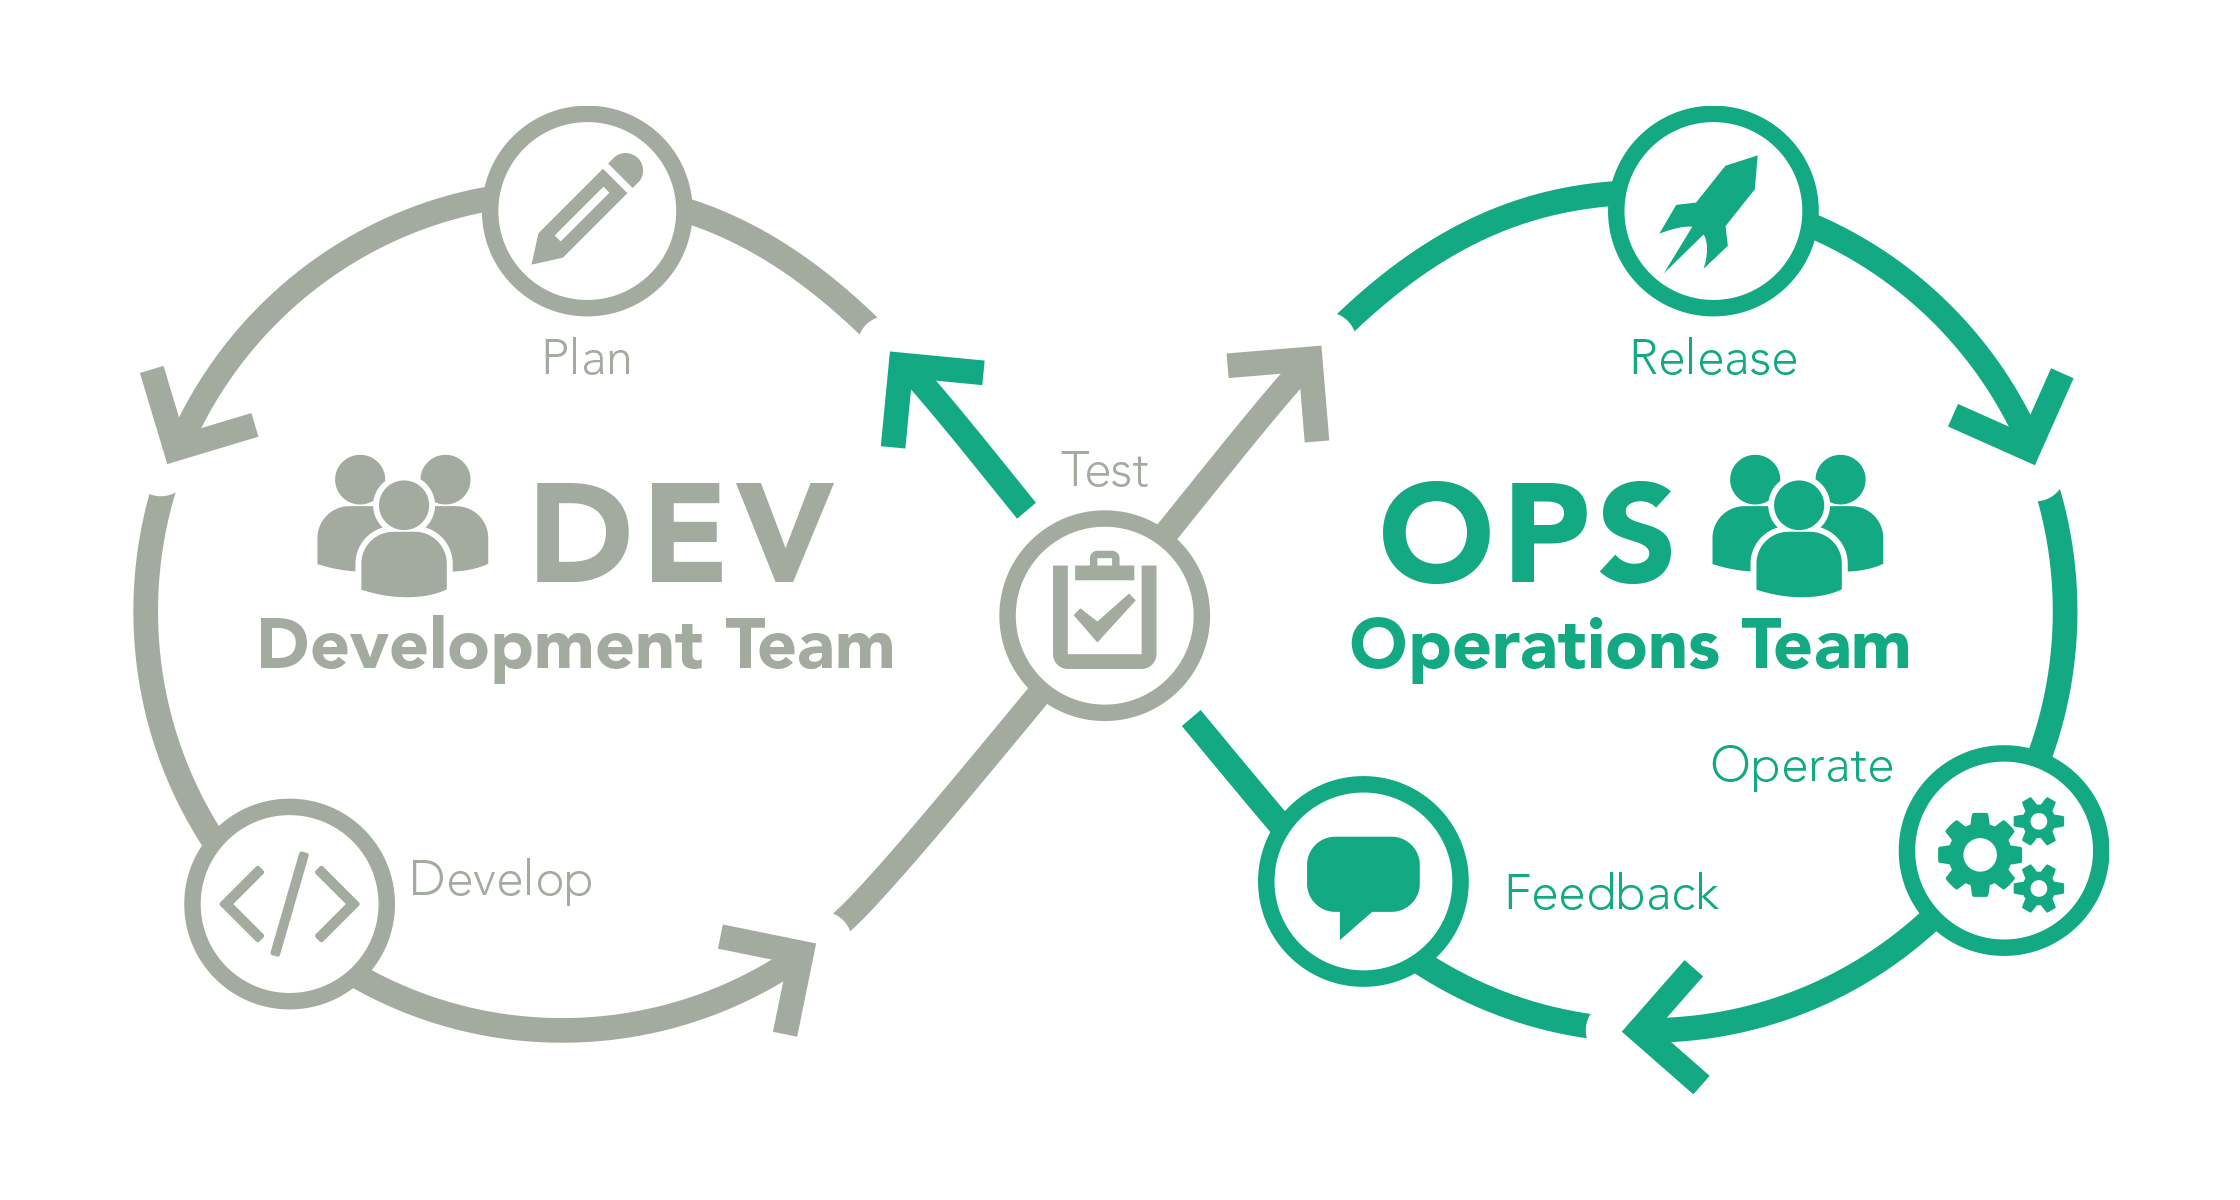
\includegraphics[scale=0.15]{Bilder/slider-realtech-devops-for-sap-acht}
    \caption{Ein Beispiel für ein DevOpsLifecycle}
\end{figure}

Hierbei wird auch auf das Shift-Left-Prinzip eingegangen. Dies beschreibt die unmittelbare Einbindung des Betriebs in die Software-Entwicklungsteams, um die betrieblichen Erfordernisse besser zu berücksichtigen und früher zu testen.

\begin{figure}[h]
    \centering
    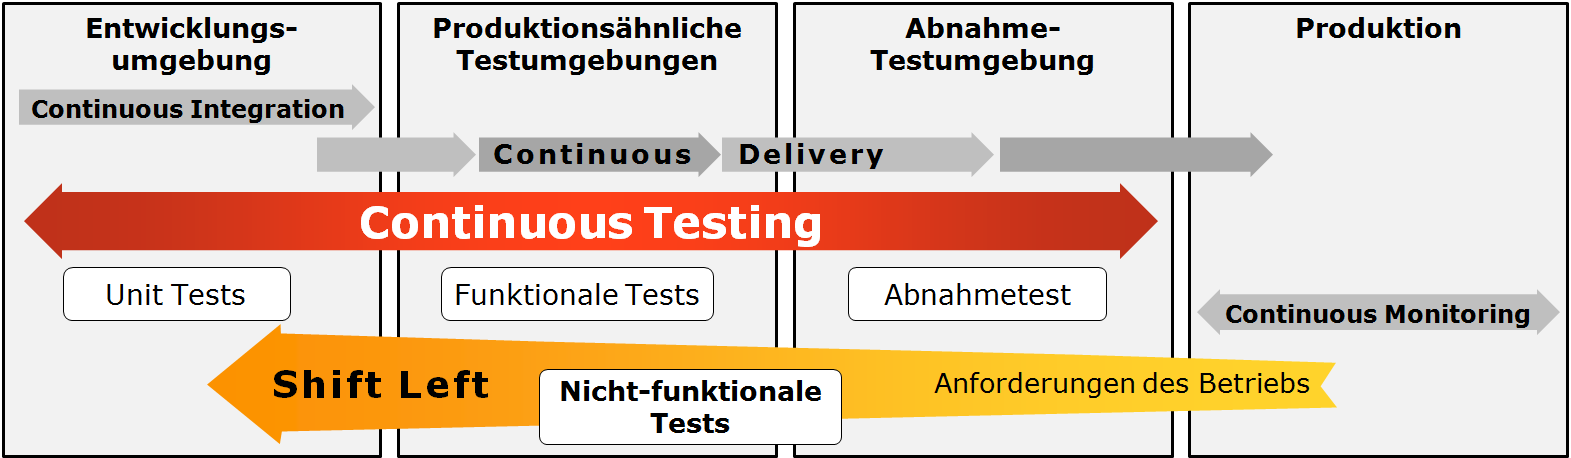
\includegraphics[scale=0.3]{Bilder/shift-left}
    \caption{Shift-Left-Prinzip}
\end{figure}

